

\section{Introduktion} %%%%%%%%%%%%%%%%%%%%%%%%%%%%%%%%%%%%%%%%%%%%%%%%%%%%%%%%%%%%
%%%%%%%%%%%% MID WAY AGENDA %%%%%%%%%%%%%%
%\begin{frame}<beamer>
%\frametitle{Simon Bjerre Krogh}
%\tableofcontents[currentsection]
%\end{frame}


% the license
\subsection{Kloakker og rensningsanlæg generelt} %%%%%%%%%%%%%%%%%%%%%%%%
\begin{frame}{Typisk opbygning af kloak ledning}{}
\vfill\vfill\centering
\begin{figure}[H]
\centering
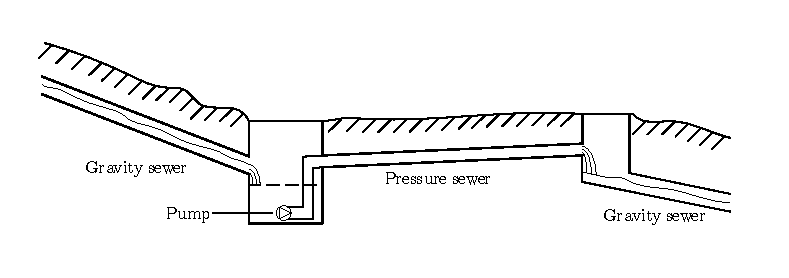
\includegraphics[width=1\textwidth]{Sections/pictures/Sewer_drawing.pdf}
\end{figure}
\vfill\vfill
\end{frame}
%
%\subsection{Rensningsanlæg} %%%%%%%%%%%%%%%%%%%%%%%%%%

\begin{frame}{Tilstande i kloakken}
\vfill\vfill\centering
\begin{itemize}
	\item<1-> Aerob $\rightarrow$ $O_2$ $\rightarrow$ $H_2O$
	\item<2-> Anaerob $\rightarrow$ $SO_4^{-2}$ $\rightarrow$ $H_2S$
	\item<3-> Anoxisk $\rightarrow$ $NO_3^-$ $\rightarrow$ $N_2$
\end{itemize}
\vfill\vfill	
\end{frame}

\begin{frame}{Udfordringer ved spildevands rensning}{}
\vfill\vfill\centering
\begin{itemize}
	\item Virksomheds besøg ved Fredericia Spildevand og Energi A/S.
	
	\begin{itemize}
		\item<1-> Større udledninger uden varsel
		\item<2-> Problemer for aerobe bakterier
		\item<3-> Andre forstyrelser
	\end{itemize}	

\end{itemize}
\vfill\vfill
\end{frame}

\subsection{Problem formulering}

\begin{frame}{Problem formulering}{}
\vfill\vfill\centering
How can a simulation environment be constructed, which mimic the behavior of a real
sewer system, where MPC is utilized as the control scheme to obtain stable sewage output
such that optimal performance can be obtained from a WWTP.
\vfill\vfill
\end{frame}

\section{System beskrivelse} %%%%%%%%%%%%%%%%%%%%%%%%%%%%%%%%%%%%%%%%%%%%%%%%%%%%%%%%%%%%%%%%%%

%\subsection{Udgangspunkt i et virkeligt setup} %%%%%%%

\begin{frame}{Udgangspunkt i et virkeligt setup}{}
%\centering
\begin{figure}[H]
\centering
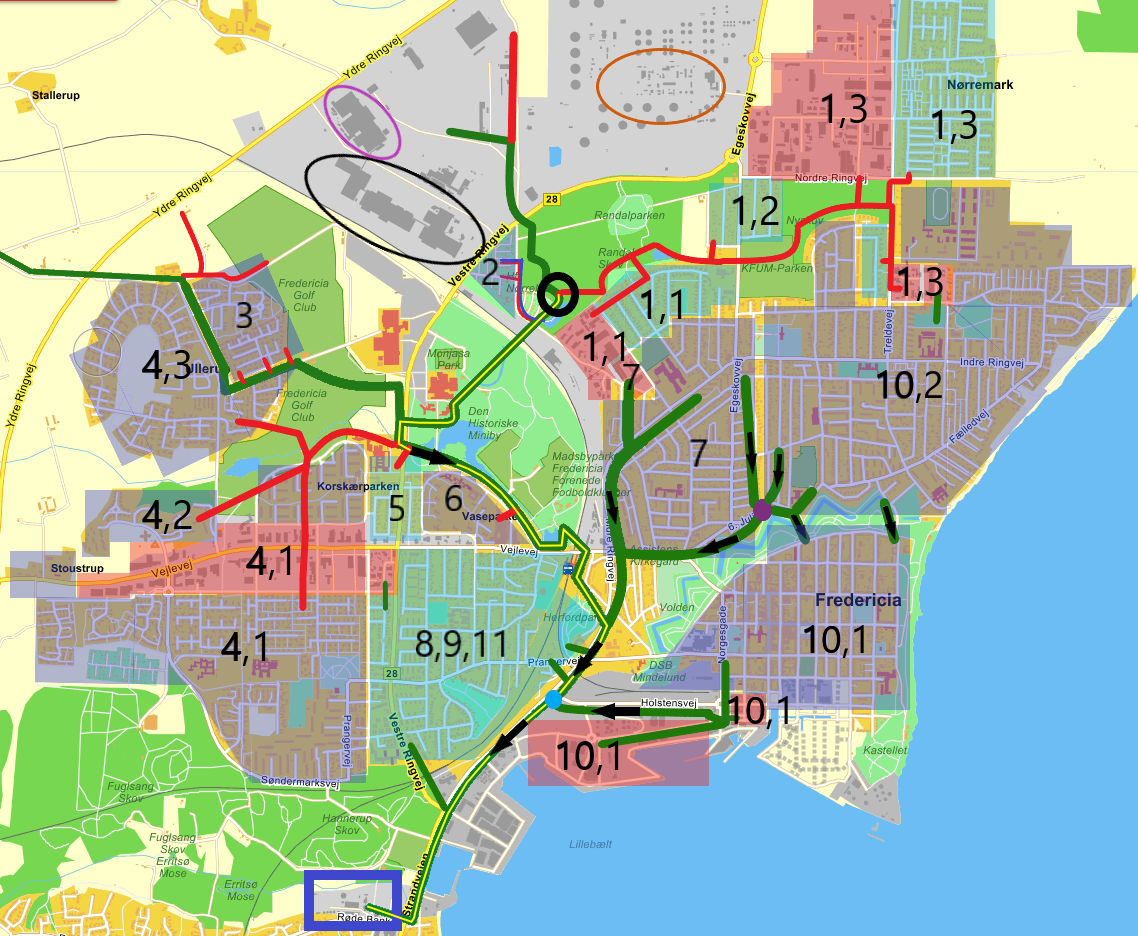
\includegraphics[width=0.7\textwidth]{Sections/pictures/kloakgrid_simplified10.png}
\end{figure}
%\vfill\vfill
\end{frame}

\begin{frame}{Udgangspunkt i et virkeligt setup}{}
\vfill\vfill\centering
\begin{itemize}
	\item Data fra industri.
	\item Flow profiler af beboelse og mindre industri.
\end{itemize}
\vfill\vfill	
\end{frame}

\subsection{Løsninger og begrænsninger}
\begin{frame}{Valg}{}
\vfill\vfill\centering
\begin{itemize}
	\item<1-> Indsættelse af tank.
	\item<2-> Afgrænse simulering til enkelt kemisk component.
	\item<3-> Runde kloak rør.
\end{itemize}
\vfill\vfill	
\end{frame}

\section{Modellering}

\begin{frame}{4 modeller}{}
	\vfill\vfill\centering
\begin{itemize}
	\item Kloak ledning.
	\item Transport af concentrat i kloak ledning.
	\item Sammenkobling af kloakledninger.
	\item Tank. 
\end{itemize}
\vfill\vfill		
\end{frame}

\begin{frame}{Kloak ledning}{Saint-Venant ligningerne}{}
	\vfill\vfill\centering
	
\begin{columns}
		\begin{column}{0.4\textwidth}
			\begin{itemize}
				\item<1-> $\dfrac{\partial A(x,t)}{\partial t} + \dfrac{\partial Q(x,t)}{\partial x}=0$
				\vspace{9mm}
				\item<2-> $\dfrac{1}{gA} \dfrac{\partial Q}{\partial t} +\dfrac{1}{gA}\dfrac{\partial}{\partial x} \left( \dfrac{Q^2}{A} \right) +
				\dfrac{\partial h}{\partial x} + S_f - S_b = 0$
				
				\vspace{9mm}
				\item<3-> Approksimationer af momentum ligningen.
				%\item<4-> Kinematisk bølge approksimation
			\end{itemize}
		\end{column}
		\begin{column}{0.48\textwidth}
			\begin{figure}[H]
				\centering
				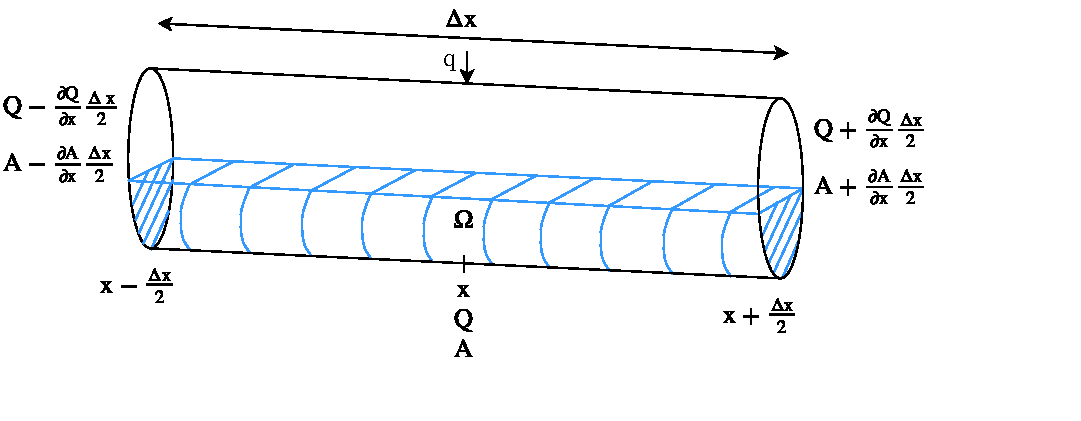
\includegraphics[width=1.2\textwidth]{Sections/pictures/continuity_open_channel.pdf}
			\end{figure}
		\end{column}
	\end{columns}
\vfill\vfill		
\end{frame}

\begin{frame}{Transport af koncentrat}{}
	\vfill\vfill\centering
\begin{columns}
	\begin{column}{0.4\textwidth}
		\begin{itemize}
			\vspace{9mm}
			\item<1-> $	A \cdot \dfrac{\partial C}{\partial t} + Q \cdot \dfrac{\partial C}{\partial x} = 0$
			\vspace{9mm}
			\item<2-> Afhænger af kendt $A$ og $Q$.
		\end{itemize}
	\end{column}
	
	\begin{column}{0.48\textwidth}
		\begin{figure}[H]
			\centering
			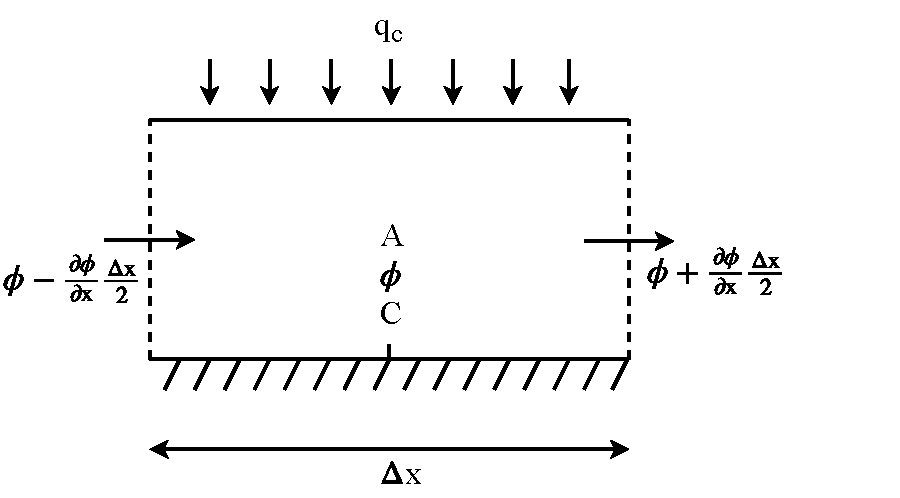
\includegraphics[width=1.1\textwidth]{Sections/pictures/poopvolume.pdf}
		\end{figure}
	\end{column}
\end{columns}


\vfill\vfill		
\end{frame}

\begin{frame}{Sammenkobling af kloak ledninger}{}
\vfill\vfill\centering
	\begin{columns}
	\begin{column}{0.4\textwidth}
		\begin{itemize}
			\vspace{9mm}
			\item<1-> $Q_3 = Q_1 + Q_2$
			\vspace{9mm}
			\item<2-> $C_3 = \dfrac{C_1 \cdot Q_1 + C_2 \cdot Q_2}{Q_1 + Q_2}$
		\end{itemize}
	\end{column}

	\begin{column}{0.48\textwidth}
		\begin{figure}[H]
			\centering
			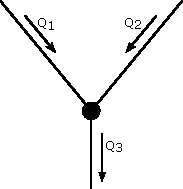
\includegraphics[width=0.7\textwidth]{Sections/pictures/interconnections.pdf}
		\end{figure}
	\end{column}
\end{columns}
\vfill\vfill		
\end{frame}

\begin{frame}{Tank}{}
\vfill\vfill\centering
	\begin{columns}
	\begin{column}{0.75\textwidth}
		\begin{itemize}
			\vspace{9mm}
			\item<1-> $\dfrac{dh(t)}{dt}=\dfrac{1}{A} \left(Q_{in}(t)-u(t) \cdot \overline Q \right)$
			\vspace{9mm}
			\item<2-> $\dfrac{dC_{tank}(t)}{dt} = \dfrac{1}{A} \left(C_{in}(t) \cdot \dfrac{Q_{in}(t)}{h(t)} - C_{tank}(t) \cdot \dfrac{Q_{out}(t)}{h(t)} \right)$
		\end{itemize}
	\end{column}

	\begin{column}{0.3\textwidth}
		\begin{figure}[H]
			\centering
			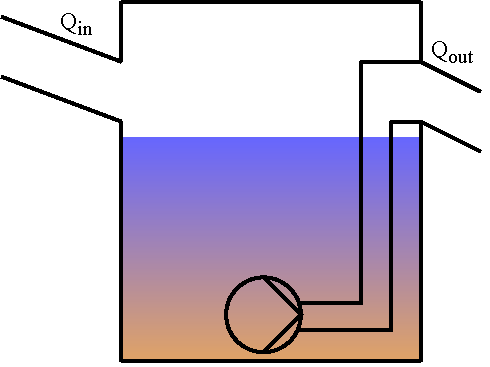
\includegraphics[width=0.9\textwidth]{Sections/pictures/reservior_with_pump.pdf}
		\end{figure}
	\end{column}
\end{columns}
\vfill\vfill		
\end{frame}
	
\section{Simulering}
\subsection{Struktur}
\begin{frame}{Tre dele}{}
\vfill\vfill\centering

\begin{itemize}
	\item \textbf{Intialisering}
	\item<1-> Opsætning af komponenter.
	\item<2-> System i steady state.
	\item<3-> \textbf{Simulering}
	\item<4-> Iterativ beregning af komponenterne
	\item<5-> \textbf{Gennemgang af resultat}
\end{itemize}

\vfill\vfill		
\end{frame}

\begin{frame}{Playback funktion}{}
\vfill\vfill\centering
		\begin{figure}[H]
			\centering
			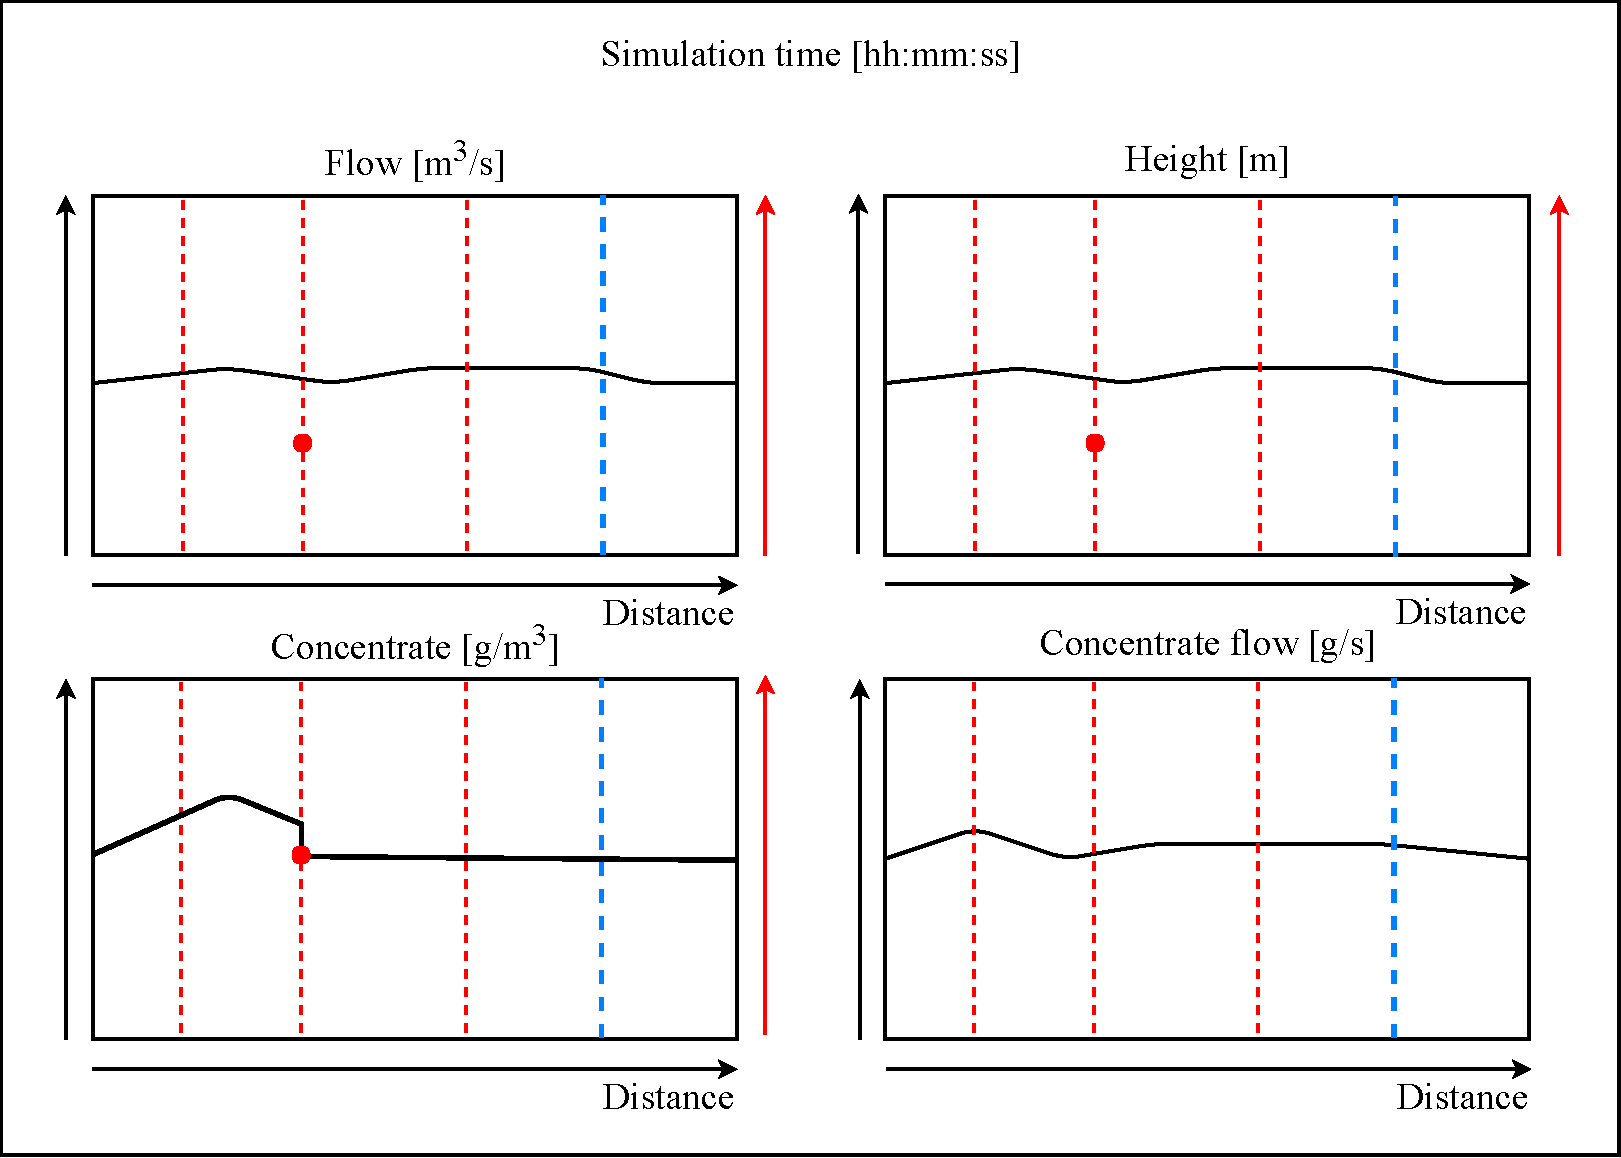
\includegraphics[width=0.7\textwidth]{Sections/pictures/display_results.pdf}
		\end{figure}
\vfill\vfill		
\end{frame}

\subsection{Preissmann}

\begin{frame}{Preissmann basic}{}
\vfill\vfill\centering
		\begin{figure}[H]
			\centering
			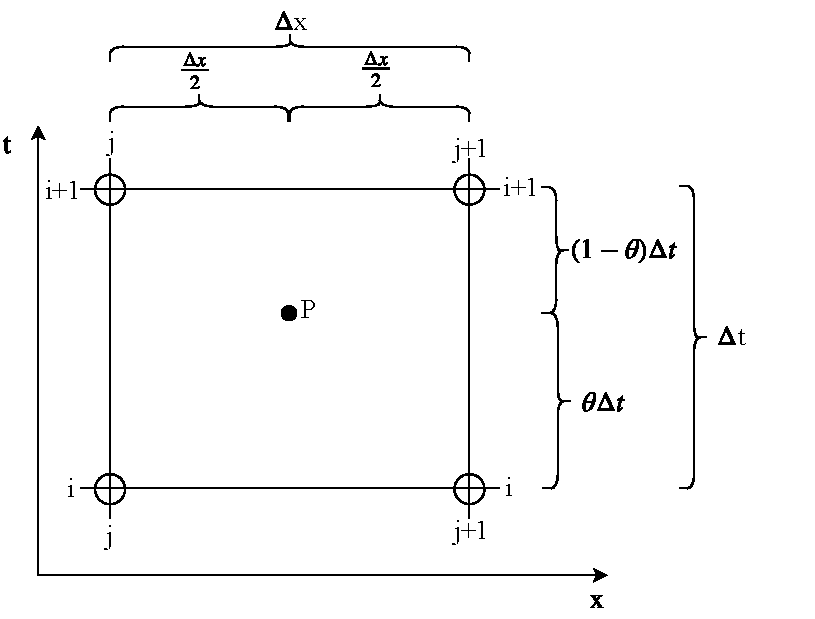
\includegraphics[width=0.7\textwidth]{Sections/pictures/preissmann_scheme.pdf}
		\end{figure}
\vfill\vfill		
\end{frame}

\begin{frame}{Preissmann iteration}{}
\vfill\vfill\centering
		\begin{figure}[H]
			\centering
			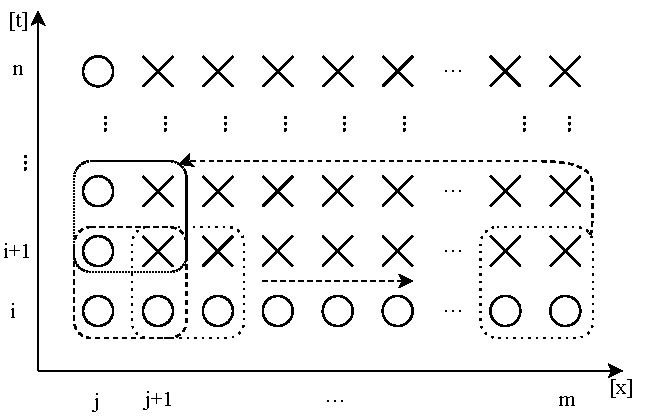
\includegraphics[width=0.7\textwidth]{Sections/pictures/preissmann_scheme_iteration.pdf}
		\end{figure}
\vfill\vfill		
\end{frame}